\documentclass[1p]{elsarticle_modified}
%\bibliographystyle{elsarticle-num}

%\usepackage[colorlinks]{hyperref}
%\usepackage{abbrmath_seonhwa} %\Abb, \Ascr, \Acal ,\Abf, \Afrak
\usepackage{amsfonts}
\usepackage{amssymb}
\usepackage{amsmath}
\usepackage{amsthm}
\usepackage{scalefnt}
\usepackage{amsbsy}
\usepackage{kotex}
\usepackage{caption}
\usepackage{subfig}
\usepackage{color}
\usepackage{graphicx}
\usepackage{xcolor} %% white, black, red, green, blue, cyan, magenta, yellow
\usepackage{float}
\usepackage{setspace}
\usepackage{hyperref}

\usepackage{tikz}
\usetikzlibrary{arrows}

\usepackage{multirow}
\usepackage{array} % fixed length table
\usepackage{hhline}

%%%%%%%%%%%%%%%%%%%%%
\makeatletter
\renewcommand*\env@matrix[1][\arraystretch]{%
	\edef\arraystretch{#1}%
	\hskip -\arraycolsep
	\let\@ifnextchar\new@ifnextchar
	\array{*\c@MaxMatrixCols c}}
\makeatother %https://tex.stackexchange.com/questions/14071/how-can-i-increase-the-line-spacing-in-a-matrix
%%%%%%%%%%%%%%%

\usepackage[normalem]{ulem}

\newcommand{\msout}[1]{\ifmmode\text{\sout{\ensuremath{#1}}}\else\sout{#1}\fi}
%SOURCE: \msout is \stkout macro in https://tex.stackexchange.com/questions/20609/strikeout-in-math-mode

\newcommand{\cancel}[1]{
	\ifmmode
	{\color{red}\msout{#1}}
	\else
	{\color{red}\sout{#1}}
	\fi
}

\newcommand{\add}[1]{
	{\color{blue}\uwave{#1}}
}

\newcommand{\replace}[2]{
	\ifmmode
	{\color{red}\msout{#1}}{\color{blue}\uwave{#2}}
	\else
	{\color{red}\sout{#1}}{\color{blue}\uwave{#2}}
	\fi
}

\newcommand{\Sol}{\mathcal{S}} %segment
\newcommand{\D}{D} %diagram
\newcommand{\A}{\mathcal{A}} %arc


%%%%%%%%%%%%%%%%%%%%%%%%%%%%%5 test

\def\sl{\operatorname{\textup{SL}}(2,\Cbb)}
\def\psl{\operatorname{\textup{PSL}}(2,\Cbb)}
\def\quan{\mkern 1mu \triangleright \mkern 1mu}

\theoremstyle{definition}
\newtheorem{thm}{Theorem}[section]
\newtheorem{prop}[thm]{Proposition}
\newtheorem{lem}[thm]{Lemma}
\newtheorem{ques}[thm]{Question}
\newtheorem{cor}[thm]{Corollary}
\newtheorem{defn}[thm]{Definition}
\newtheorem{exam}[thm]{Example}
\newtheorem{rmk}[thm]{Remark}
\newtheorem{alg}[thm]{Algorithm}

\newcommand{\I}{\sqrt{-1}}
\begin{document}

%\begin{frontmatter}
%
%\title{Boundary parabolic representations of knots up to 8 crossings}
%
%%% Group authors per affiliation:
%\author{Yunhi Cho} 
%\address{Department of Mathematics, University of Seoul, Seoul, Korea}
%\ead{yhcho@uos.ac.kr}
%
%
%\author{Seonhwa Kim} %\fnref{s_kim}}
%\address{Center for Geometry and Physics, Institute for Basic Science, Pohang, 37673, Korea}
%\ead{ryeona17@ibs.re.kr}
%
%\author{Hyuk Kim}
%\address{Department of Mathematical Sciences, Seoul National University, Seoul 08826, Korea}
%\ead{hyukkim@snu.ac.kr}
%
%\author{Seokbeom Yoon}
%\address{Department of Mathematical Sciences, Seoul National University, Seoul, 08826,  Korea}
%\ead{sbyoon15@snu.ac.kr}
%
%\begin{abstract}
%We find all boundary parabolic representation of knots up to 8 crossings.
%
%\end{abstract}
%\begin{keyword}
%    \MSC[2010] 57M25 
%\end{keyword}
%
%\end{frontmatter}

%\linenumbers
%\tableofcontents
%
\newcommand\colored[1]{\textcolor{white}{\rule[-0.35ex]{0.8em}{1.4ex}}\kern-0.8em\color{red} #1}%
%\newcommand\colored[1]{\textcolor{white}{ #1}\kern-2.17ex	\textcolor{white}{ #1}\kern-1.81ex	\textcolor{white}{ #1}\kern-2.15ex\color{red}#1	}

{\Large $\underline{12a_{0604}~(K12a_{0604})}$}

\setlength{\tabcolsep}{10pt}
\renewcommand{\arraystretch}{1.6}
\vspace{1cm}\begin{tabular}{m{100pt}>{\centering\arraybackslash}m{274pt}}
\multirow{5}{120pt}{
	\centering
	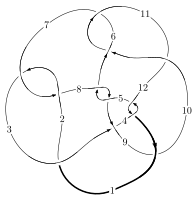
\includegraphics[width=112pt]{../../../GIT/diagram.site/Diagrams/png/1405_12a_0604.png}\\
\ \ \ A knot diagram\footnotemark}&
\allowdisplaybreaks
\textbf{Linearized knot diagam} \\
\cline{2-2}
 &
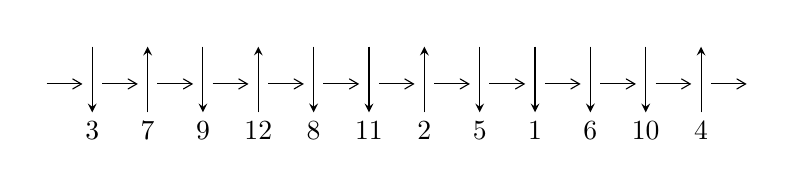
\begin{tikzpicture}[x=20pt, y=17pt]
	% nodes
	\node (C0) at (0, 0) {};
	\node (C1) at (1, 0) {};
	\node (C1U) at (1, +1) {};
	\node (C1D) at (1, -1) {3};

	\node (C2) at (2, 0) {};
	\node (C2U) at (2, +1) {};
	\node (C2D) at (2, -1) {7};

	\node (C3) at (3, 0) {};
	\node (C3U) at (3, +1) {};
	\node (C3D) at (3, -1) {9};

	\node (C4) at (4, 0) {};
	\node (C4U) at (4, +1) {};
	\node (C4D) at (4, -1) {12};

	\node (C5) at (5, 0) {};
	\node (C5U) at (5, +1) {};
	\node (C5D) at (5, -1) {8};

	\node (C6) at (6, 0) {};
	\node (C6U) at (6, +1) {};
	\node (C6D) at (6, -1) {11};

	\node (C7) at (7, 0) {};
	\node (C7U) at (7, +1) {};
	\node (C7D) at (7, -1) {2};

	\node (C8) at (8, 0) {};
	\node (C8U) at (8, +1) {};
	\node (C8D) at (8, -1) {5};

	\node (C9) at (9, 0) {};
	\node (C9U) at (9, +1) {};
	\node (C9D) at (9, -1) {1};

	\node (C10) at (10, 0) {};
	\node (C10U) at (10, +1) {};
	\node (C10D) at (10, -1) {6};

	\node (C11) at (11, 0) {};
	\node (C11U) at (11, +1) {};
	\node (C11D) at (11, -1) {10};

	\node (C12) at (12, 0) {};
	\node (C12U) at (12, +1) {};
	\node (C12D) at (12, -1) {4};
	\node (C13) at (13, 0) {};

	% arrows
	\draw[->,>={angle 60}]
	(C0) edge (C1) (C1) edge (C2) (C2) edge (C3) (C3) edge (C4) (C4) edge (C5) (C5) edge (C6) (C6) edge (C7) (C7) edge (C8) (C8) edge (C9) (C9) edge (C10) (C10) edge (C11) (C11) edge (C12) (C12) edge (C13) ;	\draw[->,>=stealth]
	(C1U) edge (C1D) (C2D) edge (C2U) (C3U) edge (C3D) (C4D) edge (C4U) (C5U) edge (C5D) (C6U) edge (C6D) (C7D) edge (C7U) (C8U) edge (C8D) (C9U) edge (C9D) (C10U) edge (C10D) (C11U) edge (C11D) (C12D) edge (C12U) ;
	\end{tikzpicture} \\
\hhline{~~} \\& 
\textbf{Solving Sequence} \\ \cline{2-2} 
 &
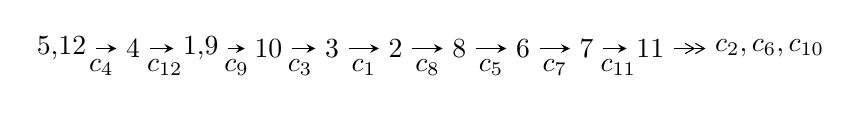
\begin{tikzpicture}[x=23pt, y=7pt]
	% node
	\node (A0) at (-1/8, 0) {5,12};
	\node (A1) at (1, 0) {4};
	\node (A2) at (33/16, 0) {1,9};
	\node (A3) at (25/8, 0) {10};
	\node (A4) at (33/8, 0) {3};
	\node (A5) at (41/8, 0) {2};
	\node (A6) at (49/8, 0) {8};
	\node (A7) at (57/8, 0) {6};
	\node (A8) at (65/8, 0) {7};
	\node (A9) at (73/8, 0) {11};
	\node (C1) at (1/2, -1) {$c_{4}$};
	\node (C2) at (3/2, -1) {$c_{12}$};
	\node (C3) at (21/8, -1) {$c_{9}$};
	\node (C4) at (29/8, -1) {$c_{3}$};
	\node (C5) at (37/8, -1) {$c_{1}$};
	\node (C6) at (45/8, -1) {$c_{8}$};
	\node (C7) at (53/8, -1) {$c_{5}$};
	\node (C8) at (61/8, -1) {$c_{7}$};
	\node (C9) at (69/8, -1) {$c_{11}$};
	\node (A10) at (11, 0) {$c_{2},c_{6},c_{10}$};

	% edge
	\draw[->,>=stealth]	
	(A0) edge (A1) (A1) edge (A2) (A2) edge (A3) (A3) edge (A4) (A4) edge (A5) (A5) edge (A6) (A6) edge (A7) (A7) edge (A8) (A8) edge (A9) ;
	\draw[->>,>={angle 60}]	
	(A9) edge (A10);
\end{tikzpicture} \\ 

\end{tabular} \\

\footnotetext{
The image of knot diagram is generated by the software ``\textbf{Draw programme}" developed by Andrew Bartholomew(\url{http://www.layer8.co.uk/maths/draw/index.htm\#Running-draw}), where we modified some parts for our purpose(\url{https://github.com/CATsTAILs/LinksPainter}).
}\phantom \\ \newline 
\centering \textbf{Ideals for irreducible components\footnotemark of $X_{\text{par}}$} 
 
\begin{align*}
I^u_{1}&=\langle 
1.06975\times10^{546} u^{142}-7.77145\times10^{546} u^{141}+\cdots+3.41807\times10^{543} b+1.40078\times10^{548},\\
\phantom{I^u_{1}}&\phantom{= \langle  }-2.07944\times10^{545} u^{142}+2.80717\times10^{546} u^{141}+\cdots+3.41807\times10^{543} a-2.16578\times10^{548},\\
\phantom{I^u_{1}}&\phantom{= \langle  }u^{143}-7 u^{142}+\cdots+3881 u-121\rangle \\
I^u_{2}&=\langle 
1318285860373840 u^{31}-1436322685985714 u^{30}+\cdots+173990609655301 b-3641781170576400,\\
\phantom{I^u_{2}}&\phantom{= \langle  }3863358201022951 u^{31}+4701671484443780 u^{30}+\cdots+173990609655301 a+5565697109234501,\\
\phantom{I^u_{2}}&\phantom{= \langle  }u^{32}+12 u^{30}+\cdots+u+1\rangle \\
\\
\end{align*}
\raggedright * 2 irreducible components of $\dim_{\mathbb{C}}=0$, with total 175 representations.\\
\footnotetext{All coefficients of polynomials are rational numbers. But the coefficients are sometimes approximated in decimal forms when there is not enough margin.}
\newpage
\renewcommand{\arraystretch}{1}
\centering \section*{I. $I^u_{1}= \langle 1.07\times10^{546} u^{142}-7.77\times10^{546} u^{141}+\cdots+3.42\times10^{543} b+1.40\times10^{548},\;-2.08\times10^{545} u^{142}+2.81\times10^{546} u^{141}+\cdots+3.42\times10^{543} a-2.17\times10^{548},\;u^{143}-7 u^{142}+\cdots+3881 u-121 \rangle$}
\flushleft \textbf{(i) Arc colorings}\\
\begin{tabular}{m{7pt} m{180pt} m{7pt} m{180pt} }
\flushright $a_{5}=$&$\begin{pmatrix}1\\0\end{pmatrix}$ \\
\flushright $a_{12}=$&$\begin{pmatrix}0\\u\end{pmatrix}$ \\
\flushright $a_{4}=$&$\begin{pmatrix}1\\u^2\end{pmatrix}$ \\
\flushright $a_{1}=$&$\begin{pmatrix}u\\u^3+u\end{pmatrix}$ \\
\flushright $a_{9}=$&$\begin{pmatrix}60.8368 u^{142}-821.273 u^{141}+\cdots-1.99321\times10^{6} u+63362.7\\-312.970 u^{142}+2273.64 u^{141}+\cdots+1.32948\times10^{6} u-40981.7\end{pmatrix}$ \\
\flushright $a_{10}=$&$\begin{pmatrix}-213.444 u^{142}+1205.05 u^{141}+\cdots-671828. u+22460.4\\-295.721 u^{142}+2356.12 u^{141}+\cdots+2.20490\times10^{6} u-69014.7\end{pmatrix}$ \\
\flushright $a_{3}=$&$\begin{pmatrix}-163.545 u^{142}+1035.16 u^{141}+\cdots-46634.6 u+2256.25\\18.3757 u^{142}-24.5616 u^{141}+\cdots+427470. u-13730.8\end{pmatrix}$ \\
\flushright $a_{2}=$&$\begin{pmatrix}152.700 u^{142}-1154.18 u^{141}+\cdots-833158. u+25921.2\\-162.336 u^{142}+1098.28 u^{141}+\cdots+315472. u-9312.22\end{pmatrix}$ \\
\flushright $a_{8}=$&$\begin{pmatrix}-252.134 u^{142}+1452.37 u^{141}+\cdots-663723. u+22381.0\\-312.970 u^{142}+2273.64 u^{141}+\cdots+1.32948\times10^{6} u-40981.7\end{pmatrix}$ \\
\flushright $a_{6}=$&$\begin{pmatrix}-347.409 u^{142}+2438.03 u^{141}+\cdots+1.10062\times10^{6} u-33534.6\\254.951 u^{142}-1425.93 u^{141}+\cdots+867942. u-28929.3\end{pmatrix}$ \\
\flushright $a_{7}=$&$\begin{pmatrix}-288.174 u^{142}+1769.85 u^{141}+\cdots-249787. u+9322.75\\-146.578 u^{142}+1355.32 u^{141}+\cdots+1.95952\times10^{6} u-61910.5\end{pmatrix}$ \\
\flushright $a_{11}=$&$\begin{pmatrix}-250.569 u^{142}+1674.41 u^{141}+\cdots+402308. u-11699.0\\278.552 u^{142}-1552.32 u^{141}+\cdots+970880. u-32344.9\end{pmatrix}$\\&\end{tabular}
\flushleft \textbf{(ii) Obstruction class $= -1$}\\~\\
\flushleft \textbf{(iii) Cusp Shapes $= -160.761 u^{142}-47.4725 u^{141}+\cdots-4.91048\times10^{6} u+157668.$}\\~\\
\newpage\renewcommand{\arraystretch}{1}
\flushleft \textbf{(iv) u-Polynomials at the component}\newline \\
\begin{tabular}{m{50pt}|m{274pt}}
Crossings & \hspace{64pt}u-Polynomials at each crossing \\
\hline $$\begin{aligned}c_{1}\end{aligned}$$&$\begin{aligned}
&u^{143}+55 u^{142}+\cdots-53 u-1
\end{aligned}$\\
\hline $$\begin{aligned}c_{2},c_{7}\end{aligned}$$&$\begin{aligned}
&u^{143}+u^{142}+\cdots-5 u+1
\end{aligned}$\\
\hline $$\begin{aligned}c_{3}\end{aligned}$$&$\begin{aligned}
&u^{143}+u^{142}+\cdots+10 u+3
\end{aligned}$\\
\hline $$\begin{aligned}c_{4},c_{12}\end{aligned}$$&$\begin{aligned}
&u^{143}+7 u^{142}+\cdots+3881 u+121
\end{aligned}$\\
\hline $$\begin{aligned}c_{5},c_{8}\end{aligned}$$&$\begin{aligned}
&u^{143}-3 u^{142}+\cdots-2753876 u+594031
\end{aligned}$\\
\hline $$\begin{aligned}c_{6},c_{10}\end{aligned}$$&$\begin{aligned}
&u^{143}- u^{142}+\cdots-1618 u+253
\end{aligned}$\\
\hline $$\begin{aligned}c_{9}\end{aligned}$$&$\begin{aligned}
&u^{143}-3 u^{142}+\cdots-48 u+1
\end{aligned}$\\
\hline $$\begin{aligned}c_{11}\end{aligned}$$&$\begin{aligned}
&u^{143}+57 u^{142}+\cdots+375838 u+64009
\end{aligned}$\\
\hline
\end{tabular}\\~\\
\newpage\renewcommand{\arraystretch}{1}
\flushleft \textbf{(v) Riley Polynomials at the component}\newline \\
\begin{tabular}{m{50pt}|m{274pt}}
Crossings & \hspace{64pt}Riley Polynomials at each crossing \\
\hline $$\begin{aligned}c_{1}\end{aligned}$$&$\begin{aligned}
&y^{143}+79 y^{142}+\cdots-1165 y-1
\end{aligned}$\\
\hline $$\begin{aligned}c_{2},c_{7}\end{aligned}$$&$\begin{aligned}
&y^{143}+55 y^{142}+\cdots-53 y-1
\end{aligned}$\\
\hline $$\begin{aligned}c_{3}\end{aligned}$$&$\begin{aligned}
&y^{143}+7 y^{142}+\cdots-338 y-9
\end{aligned}$\\
\hline $$\begin{aligned}c_{4},c_{12}\end{aligned}$$&$\begin{aligned}
&y^{143}+87 y^{142}+\cdots+8076105 y-14641
\end{aligned}$\\
\hline $$\begin{aligned}c_{5},c_{8}\end{aligned}$$&$\begin{aligned}
&y^{143}+109 y^{142}+\cdots-10735503242368 y-352872828961
\end{aligned}$\\
\hline $$\begin{aligned}c_{6},c_{10}\end{aligned}$$&$\begin{aligned}
&y^{143}-57 y^{142}+\cdots+375838 y-64009
\end{aligned}$\\
\hline $$\begin{aligned}c_{9}\end{aligned}$$&$\begin{aligned}
&y^{143}- y^{142}+\cdots+32 y-1
\end{aligned}$\\
\hline $$\begin{aligned}c_{11}\end{aligned}$$&$\begin{aligned}
&y^{143}+75 y^{142}+\cdots-771783103574 y-4097152081
\end{aligned}$\\
\hline
\end{tabular}\\~\\
\newpage\flushleft \textbf{(vi) Complex Volumes and Cusp Shapes}
$$\begin{array}{c|c|c}  
\text{Solutions to }I^u_{1}& \I (\text{vol} + \sqrt{-1}CS) & \text{Cusp shape}\\
 \hline 
\begin{aligned}
u &= -0.409876 + 0.894319 I \\
a &= \phantom{-}2.20658 + 0.13329 I \\
b &= -0.588263 - 0.919080 I\end{aligned}
 & -0.10925 - 4.11451 I & \phantom{-0.000000 } 0 \\ \hline\begin{aligned}
u &= -0.409876 - 0.894319 I \\
a &= \phantom{-}2.20658 - 0.13329 I \\
b &= -0.588263 + 0.919080 I\end{aligned}
 & -0.10925 + 4.11451 I & \phantom{-0.000000 } 0 \\ \hline\begin{aligned}
u &= \phantom{-}0.338063 + 0.961942 I \\
a &= -2.80753 + 0.27646 I \\
b &= \phantom{-}0.011443 - 1.236700 I\end{aligned}
 & \phantom{-}4.47686 + 5.62073 I & \phantom{-0.000000 } 0 \\ \hline\begin{aligned}
u &= \phantom{-}0.338063 - 0.961942 I \\
a &= -2.80753 - 0.27646 I \\
b &= \phantom{-}0.011443 + 1.236700 I\end{aligned}
 & \phantom{-}4.47686 - 5.62073 I & \phantom{-0.000000 } 0 \\ \hline\begin{aligned}
u &= -0.406563 + 0.891523 I \\
a &= \phantom{-}0.412746 + 0.380192 I \\
b &= \phantom{-}0.046954 + 0.283956 I\end{aligned}
 & \phantom{-}0.54871 - 1.77979 I & \phantom{-0.000000 } 0 \\ \hline\begin{aligned}
u &= -0.406563 - 0.891523 I \\
a &= \phantom{-}0.412746 - 0.380192 I \\
b &= \phantom{-}0.046954 - 0.283956 I\end{aligned}
 & \phantom{-}0.54871 + 1.77979 I & \phantom{-0.000000 } 0 \\ \hline\begin{aligned}
u &= \phantom{-}0.284513 + 0.922029 I \\
a &= -1.78615 - 1.23934 I \\
b &= \phantom{-}0.254594 - 1.355680 I\end{aligned}
 & \phantom{-}3.06352 + 4.33431 I & \phantom{-0.000000 } 0 \\ \hline\begin{aligned}
u &= \phantom{-}0.284513 - 0.922029 I \\
a &= -1.78615 + 1.23934 I \\
b &= \phantom{-}0.254594 + 1.355680 I\end{aligned}
 & \phantom{-}3.06352 - 4.33431 I & \phantom{-0.000000 } 0 \\ \hline\begin{aligned}
u &= -0.353741 + 0.973035 I \\
a &= \phantom{-}2.62946 + 0.61940 I \\
b &= \phantom{-}0.074561 - 1.100870 I\end{aligned}
 & \phantom{-}4.19716 - 0.40417 I & \phantom{-0.000000 } 0 \\ \hline\begin{aligned}
u &= -0.353741 - 0.973035 I \\
a &= \phantom{-}2.62946 - 0.61940 I \\
b &= \phantom{-}0.074561 + 1.100870 I\end{aligned}
 & \phantom{-}4.19716 + 0.40417 I & \phantom{-0.000000 } 0\\
 \hline 
 \end{array}$$\newpage$$\begin{array}{c|c|c}  
\text{Solutions to }I^u_{1}& \I (\text{vol} + \sqrt{-1}CS) & \text{Cusp shape}\\
 \hline 
\begin{aligned}
u &= -0.272760 + 0.921244 I \\
a &= \phantom{-}1.30511 - 1.77902 I \\
b &= -0.288482 - 1.278600 I\end{aligned}
 & \phantom{-}1.96931 - 9.26844 I & \phantom{-0.000000 } 0 \\ \hline\begin{aligned}
u &= -0.272760 - 0.921244 I \\
a &= \phantom{-}1.30511 + 1.77902 I \\
b &= -0.288482 + 1.278600 I\end{aligned}
 & \phantom{-}1.96931 + 9.26844 I & \phantom{-0.000000 } 0 \\ \hline\begin{aligned}
u &= -0.260158 + 0.907594 I \\
a &= \phantom{-}0.180844 - 0.696566 I \\
b &= \phantom{-}0.016534 - 1.256220 I\end{aligned}
 & -1.11429 - 3.32399 I & \phantom{-0.000000 } 0 \\ \hline\begin{aligned}
u &= -0.260158 - 0.907594 I \\
a &= \phantom{-}0.180844 + 0.696566 I \\
b &= \phantom{-}0.016534 + 1.256220 I\end{aligned}
 & -1.11429 + 3.32399 I & \phantom{-0.000000 } 0 \\ \hline\begin{aligned}
u &= \phantom{-}0.312150 + 0.889695 I \\
a &= -1.76098 - 0.06289 I \\
b &= \phantom{-}0.30351 - 1.41900 I\end{aligned}
 & \phantom{-}2.42259 + 4.44141 I & \phantom{-0.000000 } 0 \\ \hline\begin{aligned}
u &= \phantom{-}0.312150 - 0.889695 I \\
a &= -1.76098 + 0.06289 I \\
b &= \phantom{-}0.30351 + 1.41900 I\end{aligned}
 & \phantom{-}2.42259 - 4.44141 I & \phantom{-0.000000 } 0 \\ \hline\begin{aligned}
u &= \phantom{-}1.069750 + 0.080254 I \\
a &= \phantom{-}0.051692 - 0.443330 I \\
b &= -0.347228 - 0.619341 I\end{aligned}
 & -2.76889 + 1.32129 I & \phantom{-0.000000 } 0 \\ \hline\begin{aligned}
u &= \phantom{-}1.069750 - 0.080254 I \\
a &= \phantom{-}0.051692 + 0.443330 I \\
b &= -0.347228 + 0.619341 I\end{aligned}
 & -2.76889 - 1.32129 I & \phantom{-0.000000 } 0 \\ \hline\begin{aligned}
u &= -0.292145 + 0.870590 I \\
a &= -2.15870 - 1.12139 I \\
b &= \phantom{-}0.84953 + 1.44858 I\end{aligned}
 & \phantom{-}4.01603 - 3.90298 I & \phantom{-0.000000 } 0 \\ \hline\begin{aligned}
u &= -0.292145 - 0.870590 I \\
a &= -2.15870 + 1.12139 I \\
b &= \phantom{-}0.84953 - 1.44858 I\end{aligned}
 & \phantom{-}4.01603 + 3.90298 I & \phantom{-0.000000 } 0\\
 \hline 
 \end{array}$$\newpage$$\begin{array}{c|c|c}  
\text{Solutions to }I^u_{1}& \I (\text{vol} + \sqrt{-1}CS) & \text{Cusp shape}\\
 \hline 
\begin{aligned}
u &= \phantom{-}1.055650 + 0.239163 I \\
a &= -0.123255 + 0.371934 I \\
b &= \phantom{-}0.39225 + 1.40040 I\end{aligned}
 & \phantom{-}7.10510 - 7.25153 I & \phantom{-0.000000 } 0 \\ \hline\begin{aligned}
u &= \phantom{-}1.055650 - 0.239163 I \\
a &= -0.123255 - 0.371934 I \\
b &= \phantom{-}0.39225 - 1.40040 I\end{aligned}
 & \phantom{-}7.10510 + 7.25153 I & \phantom{-0.000000 } 0 \\ \hline\begin{aligned}
u &= -0.390050 + 0.824416 I \\
a &= \phantom{-}2.45071 + 0.42463 I \\
b &= -1.02637 - 1.33643 I\end{aligned}
 & \phantom{-}3.17089 - 9.43341 I & \phantom{-0.000000 } 0 \\ \hline\begin{aligned}
u &= -0.390050 - 0.824416 I \\
a &= \phantom{-}2.45071 - 0.42463 I \\
b &= -1.02637 + 1.33643 I\end{aligned}
 & \phantom{-}3.17089 + 9.43341 I & \phantom{-0.000000 } 0 \\ \hline\begin{aligned}
u &= \phantom{-}0.320924 + 0.849210 I \\
a &= -0.988475 - 0.694161 I \\
b &= \phantom{-}0.606579 - 0.303759 I\end{aligned}
 & -2.00670 + 0.77075 I & \phantom{-0.000000 } 0 \\ \hline\begin{aligned}
u &= \phantom{-}0.320924 - 0.849210 I \\
a &= -0.988475 + 0.694161 I \\
b &= \phantom{-}0.606579 + 0.303759 I\end{aligned}
 & -2.00670 - 0.77075 I & \phantom{-0.000000 } 0 \\ \hline\begin{aligned}
u &= \phantom{-}0.315249 + 0.848930 I \\
a &= \phantom{-}1.96950 - 1.13587 I \\
b &= -0.59718 + 1.58798 I\end{aligned}
 & \phantom{-}4.60476 - 1.50789 I & \phantom{-0.000000 } 0 \\ \hline\begin{aligned}
u &= \phantom{-}0.315249 - 0.848930 I \\
a &= \phantom{-}1.96950 + 1.13587 I \\
b &= -0.59718 - 1.58798 I\end{aligned}
 & \phantom{-}4.60476 + 1.50789 I & \phantom{-0.000000 } 0 \\ \hline\begin{aligned}
u &= \phantom{-}0.364690 + 0.825608 I \\
a &= -2.27109 + 0.55935 I \\
b &= \phantom{-}0.85536 - 1.50734 I\end{aligned}
 & \phantom{-}4.07252 + 4.30234 I & \phantom{-0.000000 } 0 \\ \hline\begin{aligned}
u &= \phantom{-}0.364690 - 0.825608 I \\
a &= -2.27109 - 0.55935 I \\
b &= \phantom{-}0.85536 + 1.50734 I\end{aligned}
 & \phantom{-}4.07252 - 4.30234 I & \phantom{-0.000000 } 0\\
 \hline 
 \end{array}$$\newpage$$\begin{array}{c|c|c}  
\text{Solutions to }I^u_{1}& \I (\text{vol} + \sqrt{-1}CS) & \text{Cusp shape}\\
 \hline 
\begin{aligned}
u &= \phantom{-}0.878292 + 0.182741 I \\
a &= \phantom{-}0.481164 + 0.015312 I \\
b &= -0.133818 + 1.198810 I\end{aligned}
 & \phantom{-}0.47134 + 5.51955 I & \phantom{-0.000000 } 0 \\ \hline\begin{aligned}
u &= \phantom{-}0.878292 - 0.182741 I \\
a &= \phantom{-}0.481164 - 0.015312 I \\
b &= -0.133818 - 1.198810 I\end{aligned}
 & \phantom{-}0.47134 - 5.51955 I & \phantom{-0.000000 } 0 \\ \hline\begin{aligned}
u &= -0.203253 + 0.866437 I \\
a &= -0.123173 + 1.053840 I \\
b &= \phantom{-}0.43068 - 1.87863 I\end{aligned}
 & \phantom{-}4.24284 + 1.56767 I & \phantom{-0.000000 } 0 \\ \hline\begin{aligned}
u &= -0.203253 - 0.866437 I \\
a &= -0.123173 - 1.053840 I \\
b &= \phantom{-}0.43068 + 1.87863 I\end{aligned}
 & \phantom{-}4.24284 - 1.56767 I & \phantom{-0.000000 } 0 \\ \hline\begin{aligned}
u &= -0.438231 + 0.769882 I \\
a &= -0.042539 - 0.958749 I \\
b &= -0.60561 + 1.59204 I\end{aligned}
 & \phantom{-}3.30529 + 5.86418 I & \phantom{-0.000000 } 0 \\ \hline\begin{aligned}
u &= -0.438231 - 0.769882 I \\
a &= -0.042539 + 0.958749 I \\
b &= -0.60561 - 1.59204 I\end{aligned}
 & \phantom{-}3.30529 - 5.86418 I & \phantom{-0.000000 } 0 \\ \hline\begin{aligned}
u &= -0.165810 + 1.108060 I \\
a &= -1.43463 + 0.11979 I \\
b &= \phantom{-}0.858673 - 0.500804 I\end{aligned}
 & -3.94404 - 0.75957 I & \phantom{-0.000000 } 0 \\ \hline\begin{aligned}
u &= -0.165810 - 1.108060 I \\
a &= -1.43463 - 0.11979 I \\
b &= \phantom{-}0.858673 + 0.500804 I\end{aligned}
 & -3.94404 + 0.75957 I & \phantom{-0.000000 } 0 \\ \hline\begin{aligned}
u &= \phantom{-}0.413134 + 0.775606 I \\
a &= \phantom{-}0.483800 - 0.990728 I \\
b &= \phantom{-}0.39448 + 1.69283 I\end{aligned}
 & \phantom{-}4.18272 - 0.89273 I & \phantom{-0.000000 } 0 \\ \hline\begin{aligned}
u &= \phantom{-}0.413134 - 0.775606 I \\
a &= \phantom{-}0.483800 + 0.990728 I \\
b &= \phantom{-}0.39448 - 1.69283 I\end{aligned}
 & \phantom{-}4.18272 + 0.89273 I & \phantom{-0.000000 } 0\\
 \hline 
 \end{array}$$\newpage$$\begin{array}{c|c|c}  
\text{Solutions to }I^u_{1}& \I (\text{vol} + \sqrt{-1}CS) & \text{Cusp shape}\\
 \hline 
\begin{aligned}
u &= -0.437260 + 1.033550 I \\
a &= \phantom{-}1.326170 - 0.096997 I \\
b &= -0.508390 - 0.296696 I\end{aligned}
 & -0.50485 - 2.73778 I & \phantom{-0.000000 } 0 \\ \hline\begin{aligned}
u &= -0.437260 - 1.033550 I \\
a &= \phantom{-}1.326170 + 0.096997 I \\
b &= -0.508390 + 0.296696 I\end{aligned}
 & -0.50485 + 2.73778 I & \phantom{-0.000000 } 0 \\ \hline\begin{aligned}
u &= \phantom{-}0.226363 + 0.846555 I \\
a &= -0.415887 + 1.046790 I \\
b &= -0.15116 - 1.92497 I\end{aligned}
 & \phantom{-}4.79803 + 4.07547 I & \phantom{-0.000000 } 0 \\ \hline\begin{aligned}
u &= \phantom{-}0.226363 - 0.846555 I \\
a &= -0.415887 - 1.046790 I \\
b &= -0.15116 + 1.92497 I\end{aligned}
 & \phantom{-}4.79803 - 4.07547 I & \phantom{-0.000000 } 0 \\ \hline\begin{aligned}
u &= \phantom{-}0.241324 + 1.104080 I \\
a &= \phantom{-}1.59405 + 0.22801 I \\
b &= -0.816497 - 0.473422 I\end{aligned}
 & -6.21474 + 5.59156 I & \phantom{-0.000000 } 0 \\ \hline\begin{aligned}
u &= \phantom{-}0.241324 - 1.104080 I \\
a &= \phantom{-}1.59405 - 0.22801 I \\
b &= -0.816497 + 0.473422 I\end{aligned}
 & -6.21474 - 5.59156 I & \phantom{-0.000000 } 0 \\ \hline\begin{aligned}
u &= -0.837615 + 0.206861 I \\
a &= -0.362293 - 0.200136 I \\
b &= -0.133056 + 1.095170 I\end{aligned}
 & \phantom{-}1.57710 - 0.73419 I & \phantom{-0.000000 } 0 \\ \hline\begin{aligned}
u &= -0.837615 - 0.206861 I \\
a &= -0.362293 + 0.200136 I \\
b &= -0.133056 - 1.095170 I\end{aligned}
 & \phantom{-}1.57710 + 0.73419 I & \phantom{-0.000000 } 0 \\ \hline\begin{aligned}
u &= -1.134430 + 0.269030 I \\
a &= \phantom{-}0.078144 + 0.348563 I \\
b &= -0.244671 + 1.380900 I\end{aligned}
 & \phantom{-}8.39956 + 0.86716 I & \phantom{-0.000000 } 0 \\ \hline\begin{aligned}
u &= -1.134430 - 0.269030 I \\
a &= \phantom{-}0.078144 - 0.348563 I \\
b &= -0.244671 - 1.380900 I\end{aligned}
 & \phantom{-}8.39956 - 0.86716 I & \phantom{-0.000000 } 0\\
 \hline 
 \end{array}$$\newpage$$\begin{array}{c|c|c}  
\text{Solutions to }I^u_{1}& \I (\text{vol} + \sqrt{-1}CS) & \text{Cusp shape}\\
 \hline 
\begin{aligned}
u &= -0.471275 + 0.687427 I \\
a &= \phantom{-}0.132408 + 0.088818 I \\
b &= -0.375328 + 1.153630 I\end{aligned}
 & \phantom{-}0.501240 + 0.405728 I & \phantom{-0.000000 } 0 \\ \hline\begin{aligned}
u &= -0.471275 - 0.687427 I \\
a &= \phantom{-}0.132408 - 0.088818 I \\
b &= -0.375328 - 1.153630 I\end{aligned}
 & \phantom{-}0.501240 - 0.405728 I & \phantom{-0.000000 } 0 \\ \hline\begin{aligned}
u &= -0.245496 + 0.793886 I \\
a &= -2.43593 - 0.88383 I \\
b &= \phantom{-}0.261695 + 0.827557 I\end{aligned}
 & -0.754882 + 0.908230 I & \phantom{-0.000000 } 0 \\ \hline\begin{aligned}
u &= -0.245496 - 0.793886 I \\
a &= -2.43593 + 0.88383 I \\
b &= \phantom{-}0.261695 - 0.827557 I\end{aligned}
 & -0.754882 - 0.908230 I & \phantom{-0.000000 } 0 \\ \hline\begin{aligned}
u &= \phantom{-}0.545388 + 1.040330 I \\
a &= -1.49961 - 0.44283 I \\
b &= \phantom{-}0.526297 - 0.666540 I\end{aligned}
 & -2.64163 + 6.12911 I & \phantom{-0.000000 } 0 \\ \hline\begin{aligned}
u &= \phantom{-}0.545388 - 1.040330 I \\
a &= -1.49961 + 0.44283 I \\
b &= \phantom{-}0.526297 + 0.666540 I\end{aligned}
 & -2.64163 - 6.12911 I & \phantom{-0.000000 } 0 \\ \hline\begin{aligned}
u &= -0.228969 + 0.771382 I \\
a &= -3.32165 - 0.26537 I \\
b &= -0.237562 + 0.919528 I\end{aligned}
 & \phantom{-}2.50374 + 6.83691 I & \phantom{-0.000000 } 0 \\ \hline\begin{aligned}
u &= -0.228969 - 0.771382 I \\
a &= -3.32165 + 0.26537 I \\
b &= -0.237562 - 0.919528 I\end{aligned}
 & \phantom{-}2.50374 - 6.83691 I & \phantom{-0.000000 } 0 \\ \hline\begin{aligned}
u &= \phantom{-}0.317671 + 0.731649 I \\
a &= \phantom{-}1.45560 - 0.01577 I \\
b &= \phantom{-}0.074825 + 1.341700 I\end{aligned}
 & \phantom{-}2.88396 - 1.52502 I & \phantom{-0.000000 } 0 \\ \hline\begin{aligned}
u &= \phantom{-}0.317671 - 0.731649 I \\
a &= \phantom{-}1.45560 + 0.01577 I \\
b &= \phantom{-}0.074825 - 1.341700 I\end{aligned}
 & \phantom{-}2.88396 + 1.52502 I & \phantom{-0.000000 } 0\\
 \hline 
 \end{array}$$\newpage$$\begin{array}{c|c|c}  
\text{Solutions to }I^u_{1}& \I (\text{vol} + \sqrt{-1}CS) & \text{Cusp shape}\\
 \hline 
\begin{aligned}
u &= \phantom{-}0.359409 + 1.147820 I \\
a &= -0.945598 - 0.607175 I \\
b &= \phantom{-}0.859936 + 0.394641 I\end{aligned}
 & -4.22663 + 1.45748 I & \phantom{-0.000000 } 0 \\ \hline\begin{aligned}
u &= \phantom{-}0.359409 - 1.147820 I \\
a &= -0.945598 + 0.607175 I \\
b &= \phantom{-}0.859936 - 0.394641 I\end{aligned}
 & -4.22663 - 1.45748 I & \phantom{-0.000000 } 0 \\ \hline\begin{aligned}
u &= -0.722483 + 0.322293 I \\
a &= \phantom{-}0.195765 - 0.150846 I \\
b &= \phantom{-}0.062615 + 0.675116 I\end{aligned}
 & \phantom{-}1.33826 - 1.49611 I & \phantom{-0.000000 } 0 \\ \hline\begin{aligned}
u &= -0.722483 - 0.322293 I \\
a &= \phantom{-}0.195765 + 0.150846 I \\
b &= \phantom{-}0.062615 - 0.675116 I\end{aligned}
 & \phantom{-}1.33826 + 1.49611 I & \phantom{-0.000000 } 0 \\ \hline\begin{aligned}
u &= \phantom{-}0.236460 + 0.751511 I \\
a &= \phantom{-}2.87982 + 0.20790 I \\
b &= \phantom{-}0.186719 + 1.083700 I\end{aligned}
 & \phantom{-}3.65906 - 1.80529 I & \phantom{-0.000000 } 0 \\ \hline\begin{aligned}
u &= \phantom{-}0.236460 - 0.751511 I \\
a &= \phantom{-}2.87982 - 0.20790 I \\
b &= \phantom{-}0.186719 - 1.083700 I\end{aligned}
 & \phantom{-}3.65906 + 1.80529 I & \phantom{-0.000000 } 0 \\ \hline\begin{aligned}
u &= \phantom{-}1.196870 + 0.202223 I \\
a &= \phantom{-}0.063492 - 0.262345 I \\
b &= -0.50768 - 1.33425 I\end{aligned}
 & \phantom{-}5.4176 - 13.1343 I & \phantom{-0.000000 } 0 \\ \hline\begin{aligned}
u &= \phantom{-}1.196870 - 0.202223 I \\
a &= \phantom{-}0.063492 + 0.262345 I \\
b &= -0.50768 + 1.33425 I\end{aligned}
 & \phantom{-}5.4176 + 13.1343 I & \phantom{-0.000000 } 0 \\ \hline\begin{aligned}
u &= \phantom{-}0.231177 + 1.200910 I \\
a &= -0.763193 - 0.537484 I \\
b &= \phantom{-}0.686748 - 0.276936 I\end{aligned}
 & -2.00485 + 1.03914 I & \phantom{-0.000000 } 0 \\ \hline\begin{aligned}
u &= \phantom{-}0.231177 - 1.200910 I \\
a &= -0.763193 + 0.537484 I \\
b &= \phantom{-}0.686748 + 0.276936 I\end{aligned}
 & -2.00485 - 1.03914 I & \phantom{-0.000000 } 0\\
 \hline 
 \end{array}$$\newpage$$\begin{array}{c|c|c}  
\text{Solutions to }I^u_{1}& \I (\text{vol} + \sqrt{-1}CS) & \text{Cusp shape}\\
 \hline 
\begin{aligned}
u &= -0.482963 + 1.137540 I \\
a &= \phantom{-}1.55705 - 0.28439 I \\
b &= -1.229440 - 0.480521 I\end{aligned}
 & -0.52541 - 1.98449 I & \phantom{-0.000000 } 0 \\ \hline\begin{aligned}
u &= -0.482963 - 1.137540 I \\
a &= \phantom{-}1.55705 + 0.28439 I \\
b &= -1.229440 + 0.480521 I\end{aligned}
 & -0.52541 + 1.98449 I & \phantom{-0.000000 } 0 \\ \hline\begin{aligned}
u &= \phantom{-}0.456095 + 1.154010 I \\
a &= -1.52828 - 0.52113 I \\
b &= \phantom{-}1.346250 - 0.170329 I\end{aligned}
 & -1.19682 + 6.81038 I & \phantom{-0.000000 } 0 \\ \hline\begin{aligned}
u &= \phantom{-}0.456095 - 1.154010 I \\
a &= -1.52828 + 0.52113 I \\
b &= \phantom{-}1.346250 + 0.170329 I\end{aligned}
 & -1.19682 - 6.81038 I & \phantom{-0.000000 } 0 \\ \hline\begin{aligned}
u &= -0.568756 + 1.104000 I \\
a &= \phantom{-}1.150150 + 0.071404 I \\
b &= -0.692463 - 0.862627 I\end{aligned}
 & -0.99003 - 4.39494 I & \phantom{-0.000000 } 0 \\ \hline\begin{aligned}
u &= -0.568756 - 1.104000 I \\
a &= \phantom{-}1.150150 - 0.071404 I \\
b &= -0.692463 + 0.862627 I\end{aligned}
 & -0.99003 + 4.39494 I & \phantom{-0.000000 } 0 \\ \hline\begin{aligned}
u &= -0.740280 + 0.136855 I \\
a &= -0.129954 - 0.652074 I \\
b &= -0.809719 + 0.541019 I\end{aligned}
 & \phantom{-}2.33926 - 2.49575 I & \phantom{-0.000000 } 0 \\ \hline\begin{aligned}
u &= -0.740280 - 0.136855 I \\
a &= -0.129954 + 0.652074 I \\
b &= -0.809719 - 0.541019 I\end{aligned}
 & \phantom{-}2.33926 + 2.49575 I & \phantom{-0.000000 } 0 \\ \hline\begin{aligned}
u &= \phantom{-}0.180699 + 1.244330 I \\
a &= \phantom{-}1.168970 + 0.372629 I \\
b &= -0.861147 - 0.548494 I\end{aligned}
 & -8.49099 - 1.77052 I & \phantom{-0.000000 } 0 \\ \hline\begin{aligned}
u &= \phantom{-}0.180699 - 1.244330 I \\
a &= \phantom{-}1.168970 - 0.372629 I \\
b &= -0.861147 + 0.548494 I\end{aligned}
 & -8.49099 + 1.77052 I & \phantom{-0.000000 } 0\\
 \hline 
 \end{array}$$\newpage$$\begin{array}{c|c|c}  
\text{Solutions to }I^u_{1}& \I (\text{vol} + \sqrt{-1}CS) & \text{Cusp shape}\\
 \hline 
\begin{aligned}
u &= \phantom{-}0.735777 + 0.089718 I \\
a &= -0.242530 - 1.024610 I \\
b &= -0.910243 + 0.037611 I\end{aligned}
 & \phantom{-}1.25246 + 7.91091 I & \phantom{-0.000000 } 0 \\ \hline\begin{aligned}
u &= \phantom{-}0.735777 - 0.089718 I \\
a &= -0.242530 + 1.024610 I \\
b &= -0.910243 - 0.037611 I\end{aligned}
 & \phantom{-}1.25246 - 7.91091 I & \phantom{-0.000000 } 0 \\ \hline\begin{aligned}
u &= \phantom{-}0.718723 + 0.090281 I \\
a &= \phantom{-}0.061850 - 0.700454 I \\
b &= \phantom{-}0.941468 + 0.264534 I\end{aligned}
 & \phantom{-}1.86135 - 2.50434 I & \phantom{-0.000000 } 0 \\ \hline\begin{aligned}
u &= \phantom{-}0.718723 - 0.090281 I \\
a &= \phantom{-}0.061850 + 0.700454 I \\
b &= \phantom{-}0.941468 - 0.264534 I\end{aligned}
 & \phantom{-}1.86135 + 2.50434 I & \phantom{-0.000000 } 0 \\ \hline\begin{aligned}
u &= -0.701316 + 0.148407 I \\
a &= \phantom{-}0.443240 - 0.848281 I \\
b &= \phantom{-}0.703410 + 0.256407 I\end{aligned}
 & \phantom{-}2.50110 - 2.58298 I & \phantom{-0.000000 } 0 \\ \hline\begin{aligned}
u &= -0.701316 - 0.148407 I \\
a &= \phantom{-}0.443240 + 0.848281 I \\
b &= \phantom{-}0.703410 - 0.256407 I\end{aligned}
 & \phantom{-}2.50110 + 2.58298 I & \phantom{-0.000000 } 0 \\ \hline\begin{aligned}
u &= \phantom{-}0.656972 + 1.106080 I \\
a &= -1.324180 - 0.360830 I \\
b &= \phantom{-}0.378346 - 0.943016 I\end{aligned}
 & -2.53310 + 6.18641 I & \phantom{-0.000000 } 0 \\ \hline\begin{aligned}
u &= \phantom{-}0.656972 - 1.106080 I \\
a &= -1.324180 + 0.360830 I \\
b &= \phantom{-}0.378346 + 0.943016 I\end{aligned}
 & -2.53310 - 6.18641 I & \phantom{-0.000000 } 0 \\ \hline\begin{aligned}
u &= \phantom{-}0.432135 + 1.221640 I \\
a &= \phantom{-}1.43229 + 0.50481 I \\
b &= -1.51857 - 0.09633 I\end{aligned}
 & -2.49900 + 12.11870 I & \phantom{-0.000000 } 0 \\ \hline\begin{aligned}
u &= \phantom{-}0.432135 - 1.221640 I \\
a &= \phantom{-}1.43229 - 0.50481 I \\
b &= -1.51857 + 0.09633 I\end{aligned}
 & -2.49900 - 12.11870 I & \phantom{-0.000000 } 0\\
 \hline 
 \end{array}$$\newpage$$\begin{array}{c|c|c}  
\text{Solutions to }I^u_{1}& \I (\text{vol} + \sqrt{-1}CS) & \text{Cusp shape}\\
 \hline 
\begin{aligned}
u &= -0.416300 + 1.229830 I \\
a &= -1.42393 + 0.27587 I \\
b &= \phantom{-}1.404400 + 0.127993 I\end{aligned}
 & -1.41094 - 6.61756 I & \phantom{-0.000000 } 0 \\ \hline\begin{aligned}
u &= -0.416300 - 1.229830 I \\
a &= -1.42393 - 0.27587 I \\
b &= \phantom{-}1.404400 - 0.127993 I\end{aligned}
 & -1.41094 + 6.61756 I & \phantom{-0.000000 } 0 \\ \hline\begin{aligned}
u &= -1.285780 + 0.195513 I \\
a &= -0.017977 - 0.267704 I \\
b &= \phantom{-}0.376873 - 1.322230 I\end{aligned}
 & \phantom{-}7.20653 + 6.59098 I & \phantom{-0.000000 } 0 \\ \hline\begin{aligned}
u &= -1.285780 - 0.195513 I \\
a &= -0.017977 + 0.267704 I \\
b &= \phantom{-}0.376873 + 1.322230 I\end{aligned}
 & \phantom{-}7.20653 - 6.59098 I & \phantom{-0.000000 } 0 \\ \hline\begin{aligned}
u &= \phantom{-}0.082506 + 1.315580 I \\
a &= -0.126343 - 0.779054 I \\
b &= \phantom{-}0.206134 + 1.137020 I\end{aligned}
 & \phantom{-}0.87338 - 2.99536 I & \phantom{-0.000000 } 0 \\ \hline\begin{aligned}
u &= \phantom{-}0.082506 - 1.315580 I \\
a &= -0.126343 + 0.779054 I \\
b &= \phantom{-}0.206134 - 1.137020 I\end{aligned}
 & \phantom{-}0.87338 + 2.99536 I & \phantom{-0.000000 } 0 \\ \hline\begin{aligned}
u &= \phantom{-}0.406803 + 1.270930 I \\
a &= \phantom{-}1.67597 - 0.65720 I \\
b &= -0.383760 + 1.160540 I\end{aligned}
 & -3.91344 + 9.88644 I & \phantom{-0.000000 } 0 \\ \hline\begin{aligned}
u &= \phantom{-}0.406803 - 1.270930 I \\
a &= \phantom{-}1.67597 + 0.65720 I \\
b &= -0.383760 - 1.160540 I\end{aligned}
 & -3.91344 - 9.88644 I & \phantom{-0.000000 } 0 \\ \hline\begin{aligned}
u &= -0.401008 + 1.276640 I \\
a &= -1.36491 - 0.77324 I \\
b &= \phantom{-}0.249487 + 0.986213 I\end{aligned}
 & -2.87317 - 4.98544 I & \phantom{-0.000000 } 0 \\ \hline\begin{aligned}
u &= -0.401008 - 1.276640 I \\
a &= -1.36491 + 0.77324 I \\
b &= \phantom{-}0.249487 - 0.986213 I\end{aligned}
 & -2.87317 + 4.98544 I & \phantom{-0.000000 } 0\\
 \hline 
 \end{array}$$\newpage$$\begin{array}{c|c|c}  
\text{Solutions to }I^u_{1}& \I (\text{vol} + \sqrt{-1}CS) & \text{Cusp shape}\\
 \hline 
\begin{aligned}
u &= -0.342743 + 1.299600 I \\
a &= \phantom{-}0.044467 - 0.667510 I \\
b &= -0.377248 + 0.026425 I\end{aligned}
 & -1.92600 - 6.31263 I & \phantom{-0.000000 } 0 \\ \hline\begin{aligned}
u &= -0.342743 - 1.299600 I \\
a &= \phantom{-}0.044467 + 0.667510 I \\
b &= -0.377248 - 0.026425 I\end{aligned}
 & -1.92600 + 6.31263 I & \phantom{-0.000000 } 0 \\ \hline\begin{aligned}
u &= -0.398657 + 1.284730 I \\
a &= -1.115220 - 0.325759 I \\
b &= \phantom{-}0.620838 + 0.618962 I\end{aligned}
 & -3.34285 - 5.46853 I & \phantom{-0.000000 } 0 \\ \hline\begin{aligned}
u &= -0.398657 - 1.284730 I \\
a &= -1.115220 + 0.325759 I \\
b &= \phantom{-}0.620838 - 0.618962 I\end{aligned}
 & -3.34285 + 5.46853 I & \phantom{-0.000000 } 0 \\ \hline\begin{aligned}
u &= \phantom{-}0.456938 + 1.266740 I \\
a &= \phantom{-}0.776209 + 0.443984 I \\
b &= -0.865885 - 0.374996 I\end{aligned}
 & -6.95043 + 6.21889 I & \phantom{-0.000000 } 0 \\ \hline\begin{aligned}
u &= \phantom{-}0.456938 - 1.266740 I \\
a &= \phantom{-}0.776209 - 0.443984 I \\
b &= -0.865885 + 0.374996 I\end{aligned}
 & -6.95043 - 6.21889 I & \phantom{-0.000000 } 0 \\ \hline\begin{aligned}
u &= \phantom{-}0.434959 + 1.285620 I \\
a &= \phantom{-}1.43122 - 0.08980 I \\
b &= -0.659534 + 1.021300 I\end{aligned}
 & -7.05884 + 3.76976 I & \phantom{-0.000000 } 0 \\ \hline\begin{aligned}
u &= \phantom{-}0.434959 - 1.285620 I \\
a &= \phantom{-}1.43122 + 0.08980 I \\
b &= -0.659534 - 1.021300 I\end{aligned}
 & -7.05884 - 3.76976 I & \phantom{-0.000000 } 0 \\ \hline\begin{aligned}
u &= \phantom{-}0.575430 + 0.266975 I \\
a &= -0.037897 + 0.468895 I \\
b &= \phantom{-}0.433601 + 0.536034 I\end{aligned}
 & -0.59991 - 1.65353 I & \phantom{-0.000000 } 0 \\ \hline\begin{aligned}
u &= \phantom{-}0.575430 - 0.266975 I \\
a &= -0.037897 - 0.468895 I \\
b &= \phantom{-}0.433601 - 0.536034 I\end{aligned}
 & -0.59991 + 1.65353 I & \phantom{-0.000000 } 0\\
 \hline 
 \end{array}$$\newpage$$\begin{array}{c|c|c}  
\text{Solutions to }I^u_{1}& \I (\text{vol} + \sqrt{-1}CS) & \text{Cusp shape}\\
 \hline 
\begin{aligned}
u &= \phantom{-}0.640001 + 1.207760 I \\
a &= \phantom{-}0.559577 + 0.506420 I \\
b &= -0.563314 + 0.742476 I\end{aligned}
 & -1.56642 - 3.03874 I & \phantom{-0.000000 } 0 \\ \hline\begin{aligned}
u &= \phantom{-}0.640001 - 1.207760 I \\
a &= \phantom{-}0.559577 - 0.506420 I \\
b &= -0.563314 - 0.742476 I\end{aligned}
 & -1.56642 + 3.03874 I & \phantom{-0.000000 } 0 \\ \hline\begin{aligned}
u &= \phantom{-}0.600167 + 1.253790 I \\
a &= -1.66359 + 0.14533 I \\
b &= \phantom{-}0.53376 - 1.44823 I\end{aligned}
 & \phantom{-}3.92573 + 13.13200 I & \phantom{-0.000000 } 0 \\ \hline\begin{aligned}
u &= \phantom{-}0.600167 - 1.253790 I \\
a &= -1.66359 - 0.14533 I \\
b &= \phantom{-}0.53376 + 1.44823 I\end{aligned}
 & \phantom{-}3.92573 - 13.13200 I & \phantom{-0.000000 } 0 \\ \hline\begin{aligned}
u &= -0.625862 + 1.258890 I \\
a &= \phantom{-}1.50855 + 0.17248 I \\
b &= -0.41626 - 1.41135 I\end{aligned}
 & \phantom{-}5.26206 - 7.02890 I & \phantom{-0.000000 } 0 \\ \hline\begin{aligned}
u &= -0.625862 - 1.258890 I \\
a &= \phantom{-}1.50855 - 0.17248 I \\
b &= -0.41626 + 1.41135 I\end{aligned}
 & \phantom{-}5.26206 + 7.02890 I & \phantom{-0.000000 } 0 \\ \hline\begin{aligned}
u &= \phantom{-}1.20516 + 0.78491 I \\
a &= -0.256023 - 0.419927 I \\
b &= -0.208482 - 0.982709 I\end{aligned}
 & -1.91798 - 3.89604 I & \phantom{-0.000000 } 0 \\ \hline\begin{aligned}
u &= \phantom{-}1.20516 - 0.78491 I \\
a &= -0.256023 + 0.419927 I \\
b &= -0.208482 + 0.982709 I\end{aligned}
 & -1.91798 + 3.89604 I & \phantom{-0.000000 } 0 \\ \hline\begin{aligned}
u &= \phantom{-}0.196974 + 0.514065 I \\
a &= \phantom{-}0.21440 + 2.38937 I \\
b &= \phantom{-}0.034405 + 1.403400 I\end{aligned}
 & \phantom{-}5.76837 - 2.72073 I & \phantom{-0.000000 } 0 \\ \hline\begin{aligned}
u &= \phantom{-}0.196974 - 0.514065 I \\
a &= \phantom{-}0.21440 - 2.38937 I \\
b &= \phantom{-}0.034405 - 1.403400 I\end{aligned}
 & \phantom{-}5.76837 + 2.72073 I & \phantom{-0.000000 } 0\\
 \hline 
 \end{array}$$\newpage$$\begin{array}{c|c|c}  
\text{Solutions to }I^u_{1}& \I (\text{vol} + \sqrt{-1}CS) & \text{Cusp shape}\\
 \hline 
\begin{aligned}
u &= \phantom{-}0.63774 + 1.31072 I \\
a &= \phantom{-}1.53924 - 0.09161 I \\
b &= -0.66789 + 1.46266 I\end{aligned}
 & \phantom{-}1.9240 + 19.5341 I & \phantom{-0.000000 } 0 \\ \hline\begin{aligned}
u &= \phantom{-}0.63774 - 1.31072 I \\
a &= \phantom{-}1.53924 + 0.09161 I \\
b &= -0.66789 - 1.46266 I\end{aligned}
 & \phantom{-}1.9240 - 19.5341 I & \phantom{-0.000000 } 0 \\ \hline\begin{aligned}
u &= \phantom{-}0.72419 + 1.26731 I \\
a &= \phantom{-}1.180070 + 0.220824 I \\
b &= -0.459596 + 1.206970 I\end{aligned}
 & -4.17506 + 11.02990 I & \phantom{-0.000000 } 0 \\ \hline\begin{aligned}
u &= \phantom{-}0.72419 - 1.26731 I \\
a &= \phantom{-}1.180070 - 0.220824 I \\
b &= -0.459596 - 1.206970 I\end{aligned}
 & -4.17506 - 11.02990 I & \phantom{-0.000000 } 0 \\ \hline\begin{aligned}
u &= -0.65578 + 1.32482 I \\
a &= -1.400500 - 0.122714 I \\
b &= \phantom{-}0.56364 + 1.46038 I\end{aligned}
 & \phantom{-}3.63866 - 13.25200 I & \phantom{-0.000000 } 0 \\ \hline\begin{aligned}
u &= -0.65578 - 1.32482 I \\
a &= -1.400500 + 0.122714 I \\
b &= \phantom{-}0.56364 - 1.46038 I\end{aligned}
 & \phantom{-}3.63866 + 13.25200 I & \phantom{-0.000000 } 0 \\ \hline\begin{aligned}
u &= \phantom{-}1.08751 + 1.00446 I \\
a &= \phantom{-}0.352079 + 0.436032 I \\
b &= -0.050799 + 1.070720 I\end{aligned}
 & -1.52156 + 0.34717 I & \phantom{-0.000000 } 0 \\ \hline\begin{aligned}
u &= \phantom{-}1.08751 - 1.00446 I \\
a &= \phantom{-}0.352079 - 0.436032 I \\
b &= -0.050799 - 1.070720 I\end{aligned}
 & -1.52156 - 0.34717 I & \phantom{-0.000000 } 0 \\ \hline\begin{aligned}
u &= \phantom{-}0.69981 + 1.33953 I \\
a &= -0.298017 + 0.249932 I \\
b &= \phantom{-}0.068402 - 0.830064 I\end{aligned}
 & -2.56190 + 0.14422 I & \phantom{-0.000000 } 0 \\ \hline\begin{aligned}
u &= \phantom{-}0.69981 - 1.33953 I \\
a &= -0.298017 - 0.249932 I \\
b &= \phantom{-}0.068402 + 0.830064 I\end{aligned}
 & -2.56190 - 0.14422 I & \phantom{-0.000000 } 0\\
 \hline 
 \end{array}$$\newpage$$\begin{array}{c|c|c}  
\text{Solutions to }I^u_{1}& \I (\text{vol} + \sqrt{-1}CS) & \text{Cusp shape}\\
 \hline 
\begin{aligned}
u &= -0.90424 + 1.22717 I \\
a &= \phantom{-}0.757080 - 0.103344 I \\
b &= -0.014427 - 1.094330 I\end{aligned}
 & \phantom{-}2.49620 - 1.93857 I & \phantom{-0.000000 } 0 \\ \hline\begin{aligned}
u &= -0.90424 - 1.22717 I \\
a &= \phantom{-}0.757080 + 0.103344 I \\
b &= -0.014427 + 1.094330 I\end{aligned}
 & \phantom{-}2.49620 + 1.93857 I & \phantom{-0.000000 } 0 \\ \hline\begin{aligned}
u &= -0.243710 + 0.390674 I \\
a &= \phantom{-}0.89579 + 2.15684 I \\
b &= \phantom{-}0.100698 + 1.384360 I\end{aligned}
 & \phantom{-}5.68760 - 2.65348 I & \phantom{-0.000000 } 0 \\ \hline\begin{aligned}
u &= -0.243710 - 0.390674 I \\
a &= \phantom{-}0.89579 - 2.15684 I \\
b &= \phantom{-}0.100698 - 1.384360 I\end{aligned}
 & \phantom{-}5.68760 + 2.65348 I & \phantom{-0.000000 } 0 \\ \hline\begin{aligned}
u &= \phantom{-}0.282821 + 0.252122 I \\
a &= \phantom{-}1.97455 - 1.43823 I \\
b &= -0.529064 - 0.085417 I\end{aligned}
 & -3.68479 - 3.43622 I & -13.0881 + 5.6130 I \\ \hline\begin{aligned}
u &= \phantom{-}0.282821 - 0.252122 I \\
a &= \phantom{-}1.97455 + 1.43823 I \\
b &= -0.529064 + 0.085417 I\end{aligned}
 & -3.68479 + 3.43622 I & -13.0881 - 5.6130 I \\ \hline\begin{aligned}
u &= -0.89403 + 1.38947 I \\
a &= -0.696598 + 0.049512 I \\
b &= \phantom{-}0.178143 + 1.252320 I\end{aligned}
 & \phantom{-}2.20239 - 6.88117 I & \phantom{-0.000000 } 0 \\ \hline\begin{aligned}
u &= -0.89403 - 1.38947 I \\
a &= -0.696598 - 0.049512 I \\
b &= \phantom{-}0.178143 - 1.252320 I\end{aligned}
 & \phantom{-}2.20239 + 6.88117 I & \phantom{-0.000000 } 0 \\ \hline\begin{aligned}
u &= -0.49358 + 1.57840 I \\
a &= -0.564919 - 0.182390 I \\
b &= \phantom{-}0.491350 + 1.069500 I\end{aligned}
 & \phantom{-}0.15945 - 3.37795 I & \phantom{-0.000000 } 0 \\ \hline\begin{aligned}
u &= -0.49358 - 1.57840 I \\
a &= -0.564919 + 0.182390 I \\
b &= \phantom{-}0.491350 - 1.069500 I\end{aligned}
 & \phantom{-}0.15945 + 3.37795 I & \phantom{-0.000000 } 0\\
 \hline 
 \end{array}$$\newpage$$\begin{array}{c|c|c}  
\text{Solutions to }I^u_{1}& \I (\text{vol} + \sqrt{-1}CS) & \text{Cusp shape}\\
 \hline 
\begin{aligned}
u &= -0.01391 + 1.90024 I \\
a &= \phantom{-}0.175776 + 0.240003 I \\
b &= -0.343885 - 0.832877 I\end{aligned}
 & -1.49379 - 6.94000 I & \phantom{-0.000000 } 0 \\ \hline\begin{aligned}
u &= -0.01391 - 1.90024 I \\
a &= \phantom{-}0.175776 - 0.240003 I \\
b &= -0.343885 + 0.832877 I\end{aligned}
 & -1.49379 + 6.94000 I & \phantom{-0.000000 } 0 \\ \hline\begin{aligned}
u &= \phantom{-}0.0410644\phantom{ +0.000000I} \\
a &= \phantom{-}13.9495\phantom{ +0.000000I} \\
b &= \phantom{-}0.475715\phantom{ +0.000000I}\end{aligned}
 & -1.11541\phantom{ +0.000000I} & -9.18970\phantom{ +0.000000I}\\
 \hline 
 \end{array}$$\newpage\newpage\renewcommand{\arraystretch}{1}
\centering \section*{II. $I^u_{2}= \langle 1.32\times10^{15} u^{31}-1.44\times10^{15} u^{30}+\cdots+1.74\times10^{14} b-3.64\times10^{15},\;3.86\times10^{15} u^{31}+4.70\times10^{15} u^{30}+\cdots+1.74\times10^{14} a+5.57\times10^{15},\;u^{32}+12 u^{30}+\cdots+u+1 \rangle$}
\flushleft \textbf{(i) Arc colorings}\\
\begin{tabular}{m{7pt} m{180pt} m{7pt} m{180pt} }
\flushright $a_{5}=$&$\begin{pmatrix}1\\0\end{pmatrix}$ \\
\flushright $a_{12}=$&$\begin{pmatrix}0\\u\end{pmatrix}$ \\
\flushright $a_{4}=$&$\begin{pmatrix}1\\u^2\end{pmatrix}$ \\
\flushright $a_{1}=$&$\begin{pmatrix}u\\u^3+u\end{pmatrix}$ \\
\flushright $a_{9}=$&$\begin{pmatrix}-22.2044 u^{31}-27.0226 u^{30}+\cdots-82.7795 u-31.9885\\-7.57676 u^{31}+8.25517 u^{30}+\cdots+20.9332 u+20.9309\end{pmatrix}$ \\
\flushright $a_{10}=$&$\begin{pmatrix}-23.9645 u^{31}-19.3118 u^{30}+\cdots-60.3591 u-15.6485\\-4.78512 u^{31}+14.1490 u^{30}+\cdots+37.4030 u+29.5601\end{pmatrix}$ \\
\flushright $a_{3}=$&$\begin{pmatrix}4.17572 u^{31}-10.7882 u^{30}+\cdots+10.9108 u-10.7176\\- u^{30}-11 u^{28}+\cdots-13 u^2- u\end{pmatrix}$ \\
\flushright $a_{2}=$&$\begin{pmatrix}-5.84615 u^{31}-7.99209 u^{30}+\cdots-11.4592 u-11.8864\\1.20910 u^{31}+0.211125 u^{30}+\cdots+4.82395 u+1.86061\end{pmatrix}$ \\
\flushright $a_{8}=$&$\begin{pmatrix}-29.7812 u^{31}-18.7674 u^{30}+\cdots-61.8463 u-11.0576\\-7.57676 u^{31}+8.25517 u^{30}+\cdots+20.9332 u+20.9309\end{pmatrix}$ \\
\flushright $a_{6}=$&$\begin{pmatrix}-17.9894 u^{31}+1.07993 u^{30}+\cdots-32.2027 u+7.83473\\6.90542 u^{31}+4.92672 u^{30}+\cdots+29.7416 u+3.84679\end{pmatrix}$ \\
\flushright $a_{7}=$&$\begin{pmatrix}-53.1412 u^{31}+6.43759 u^{30}+\cdots-38.3877 u+30.4021\\-8.53271 u^{31}+17.5380 u^{30}+\cdots+33.7148 u+25.3631\end{pmatrix}$ \\
\flushright $a_{11}=$&$\begin{pmatrix}3.36852 u^{31}-4.41806 u^{30}+\cdots-0.241384 u-2.69627\\3.87158 u^{31}+12.9957 u^{30}+\cdots+42.2939 u+26.6186\end{pmatrix}$\\&\end{tabular}
\flushleft \textbf{(ii) Obstruction class $= 1$}\\~\\
\flushleft \textbf{(iii) Cusp Shapes $= -\frac{664759526927211}{173990609655301} u^{31}-\frac{122349895792680}{173990609655301} u^{30}+\cdots+\frac{1458028469222772}{173990609655301} u+\frac{317711536962977}{173990609655301}$}\\~\\
\newpage\renewcommand{\arraystretch}{1}
\flushleft \textbf{(iv) u-Polynomials at the component}\newline \\
\begin{tabular}{m{50pt}|m{274pt}}
Crossings & \hspace{64pt}u-Polynomials at each crossing \\
\hline $$\begin{aligned}c_{1}\end{aligned}$$&$\begin{aligned}
&u^{32}-16 u^{31}+\cdots-17 u+1
\end{aligned}$\\
\hline $$\begin{aligned}c_{2}\end{aligned}$$&$\begin{aligned}
&u^{32}+8 u^{30}+\cdots+u+1
\end{aligned}$\\
\hline $$\begin{aligned}c_{3}\end{aligned}$$&$\begin{aligned}
&u^{32}+2 u^{30}+\cdots+4 u+1
\end{aligned}$\\
\hline $$\begin{aligned}c_{4}\end{aligned}$$&$\begin{aligned}
&u^{32}+12 u^{30}+\cdots+u+1
\end{aligned}$\\
\hline $$\begin{aligned}c_{5}\end{aligned}$$&$\begin{aligned}
&u^{32}-2 u^{31}+\cdots+10 u^2+1
\end{aligned}$\\
\hline $$\begin{aligned}c_{6}\end{aligned}$$&$\begin{aligned}
&u^{32}-8 u^{30}+\cdots-2 u+1
\end{aligned}$\\
\hline $$\begin{aligned}c_{7}\end{aligned}$$&$\begin{aligned}
&u^{32}+8 u^{30}+\cdots- u+1
\end{aligned}$\\
\hline $$\begin{aligned}c_{8}\end{aligned}$$&$\begin{aligned}
&u^{32}+2 u^{31}+\cdots+10 u^2+1
\end{aligned}$\\
\hline $$\begin{aligned}c_{9}\end{aligned}$$&$\begin{aligned}
&u^{32}-6 u^{31}+\cdots+2 u^2+1
\end{aligned}$\\
\hline $$\begin{aligned}c_{10}\end{aligned}$$&$\begin{aligned}
&u^{32}-8 u^{30}+\cdots+2 u+1
\end{aligned}$\\
\hline $$\begin{aligned}c_{11}\end{aligned}$$&$\begin{aligned}
&u^{32}+16 u^{31}+\cdots+18 u+1
\end{aligned}$\\
\hline $$\begin{aligned}c_{12}\end{aligned}$$&$\begin{aligned}
&u^{32}+12 u^{30}+\cdots- u+1
\end{aligned}$\\
\hline
\end{tabular}\\~\\
\newpage\renewcommand{\arraystretch}{1}
\flushleft \textbf{(v) Riley Polynomials at the component}\newline \\
\begin{tabular}{m{50pt}|m{274pt}}
Crossings & \hspace{64pt}Riley Polynomials at each crossing \\
\hline $$\begin{aligned}c_{1}\end{aligned}$$&$\begin{aligned}
&y^{32}+12 y^{31}+\cdots+13 y+1
\end{aligned}$\\
\hline $$\begin{aligned}c_{2},c_{7}\end{aligned}$$&$\begin{aligned}
&y^{32}+16 y^{31}+\cdots+17 y+1
\end{aligned}$\\
\hline $$\begin{aligned}c_{3}\end{aligned}$$&$\begin{aligned}
&y^{32}+4 y^{31}+\cdots+2 y+1
\end{aligned}$\\
\hline $$\begin{aligned}c_{4},c_{12}\end{aligned}$$&$\begin{aligned}
&y^{32}+24 y^{31}+\cdots+27 y+1
\end{aligned}$\\
\hline $$\begin{aligned}c_{5},c_{8}\end{aligned}$$&$\begin{aligned}
&y^{32}+30 y^{31}+\cdots+20 y+1
\end{aligned}$\\
\hline $$\begin{aligned}c_{6},c_{10}\end{aligned}$$&$\begin{aligned}
&y^{32}-16 y^{31}+\cdots-18 y+1
\end{aligned}$\\
\hline $$\begin{aligned}c_{9}\end{aligned}$$&$\begin{aligned}
&y^{32}+8 y^{30}+\cdots+4 y+1
\end{aligned}$\\
\hline $$\begin{aligned}c_{11}\end{aligned}$$&$\begin{aligned}
&y^{32}+16 y^{31}+\cdots-2 y+1
\end{aligned}$\\
\hline
\end{tabular}\\~\\
\newpage\flushleft \textbf{(vi) Complex Volumes and Cusp Shapes}
$$\begin{array}{c|c|c}  
\text{Solutions to }I^u_{2}& \I (\text{vol} + \sqrt{-1}CS) & \text{Cusp shape}\\
 \hline 
\begin{aligned}
u &= \phantom{-}0.377002 + 0.860470 I \\
a &= \phantom{-}1.018800 - 0.187235 I \\
b &= \phantom{-}0.219916 + 1.383980 I\end{aligned}
 & \phantom{-}2.76714 - 0.89506 I & -5.83861 - 4.76994 I \\ \hline\begin{aligned}
u &= \phantom{-}0.377002 - 0.860470 I \\
a &= \phantom{-}1.018800 + 0.187235 I \\
b &= \phantom{-}0.219916 - 1.383980 I\end{aligned}
 & \phantom{-}2.76714 + 0.89506 I & -5.83861 + 4.76994 I \\ \hline\begin{aligned}
u &= \phantom{-}0.418834 + 1.010070 I \\
a &= -1.42074 + 0.20749 I \\
b &= \phantom{-}0.20725 - 1.40604 I\end{aligned}
 & \phantom{-}2.80871 + 5.14491 I & -2.17318 - 8.84355 I \\ \hline\begin{aligned}
u &= \phantom{-}0.418834 - 1.010070 I \\
a &= -1.42074 - 0.20749 I \\
b &= \phantom{-}0.20725 + 1.40604 I\end{aligned}
 & \phantom{-}2.80871 - 5.14491 I & -2.17318 + 8.84355 I \\ \hline\begin{aligned}
u &= \phantom{-}0.203515 + 0.870967 I \\
a &= -2.64540 - 0.11143 I \\
b &= \phantom{-}0.48543 - 1.35345 I\end{aligned}
 & \phantom{-}3.16341 + 3.49472 I & -3.10019 + 1.18656 I \\ \hline\begin{aligned}
u &= \phantom{-}0.203515 - 0.870967 I \\
a &= -2.64540 + 0.11143 I \\
b &= \phantom{-}0.48543 + 1.35345 I\end{aligned}
 & \phantom{-}3.16341 - 3.49472 I & -3.10019 - 1.18656 I \\ \hline\begin{aligned}
u &= -0.587384 + 0.953739 I \\
a &= \phantom{-}1.31554 - 0.73873 I \\
b &= -0.560197 - 0.407437 I\end{aligned}
 & -3.32326 - 5.79350 I & -12.88067 + 4.76334 I \\ \hline\begin{aligned}
u &= -0.587384 - 0.953739 I \\
a &= \phantom{-}1.31554 + 0.73873 I \\
b &= -0.560197 + 0.407437 I\end{aligned}
 & -3.32326 + 5.79350 I & -12.88067 - 4.76334 I \\ \hline\begin{aligned}
u &= \phantom{-}0.471154 + 1.030510 I \\
a &= -1.50990 - 0.23394 I \\
b &= \phantom{-}0.897386 - 0.457167 I\end{aligned}
 & -1.46713 + 2.66367 I & -9.37615 - 3.62773 I \\ \hline\begin{aligned}
u &= \phantom{-}0.471154 - 1.030510 I \\
a &= -1.50990 + 0.23394 I \\
b &= \phantom{-}0.897386 + 0.457167 I\end{aligned}
 & -1.46713 - 2.66367 I & -9.37615 + 3.62773 I\\
 \hline 
 \end{array}$$\newpage$$\begin{array}{c|c|c}  
\text{Solutions to }I^u_{2}& \I (\text{vol} + \sqrt{-1}CS) & \text{Cusp shape}\\
 \hline 
\begin{aligned}
u &= -0.149428 + 0.798777 I \\
a &= \phantom{-}2.85577 - 0.67738 I \\
b &= -0.535357 - 1.206510 I\end{aligned}
 & \phantom{-}2.22534 - 8.20210 I & -4.23687 + 6.52948 I \\ \hline\begin{aligned}
u &= -0.149428 - 0.798777 I \\
a &= \phantom{-}2.85577 + 0.67738 I \\
b &= -0.535357 + 1.206510 I\end{aligned}
 & \phantom{-}2.22534 + 8.20210 I & -4.23687 - 6.52948 I \\ \hline\begin{aligned}
u &= -0.991072 + 0.661101 I \\
a &= -0.019774 - 0.607455 I \\
b &= -0.215493 - 0.674465 I\end{aligned}
 & -2.55638 + 2.43576 I & -11.15253 - 3.40731 I \\ \hline\begin{aligned}
u &= -0.991072 - 0.661101 I \\
a &= -0.019774 + 0.607455 I \\
b &= -0.215493 + 0.674465 I\end{aligned}
 & -2.55638 - 2.43576 I & -11.15253 + 3.40731 I \\ \hline\begin{aligned}
u &= \phantom{-}0.089956 + 0.763984 I \\
a &= \phantom{-}1.069490 - 0.511674 I \\
b &= -0.07793 + 1.68527 I\end{aligned}
 & \phantom{-}4.71007 - 2.91911 I & -2.46966 + 3.28243 I \\ \hline\begin{aligned}
u &= \phantom{-}0.089956 - 0.763984 I \\
a &= \phantom{-}1.069490 + 0.511674 I \\
b &= -0.07793 - 1.68527 I\end{aligned}
 & \phantom{-}4.71007 + 2.91911 I & -2.46966 - 3.28243 I \\ \hline\begin{aligned}
u &= -0.011716 + 0.726969 I \\
a &= -1.19402 - 0.85169 I \\
b &= \phantom{-}0.33192 + 1.67681 I\end{aligned}
 & \phantom{-}4.39632 - 2.40676 I & -1.83539 + 3.91389 I \\ \hline\begin{aligned}
u &= -0.011716 - 0.726969 I \\
a &= -1.19402 + 0.85169 I \\
b &= \phantom{-}0.33192 - 1.67681 I\end{aligned}
 & \phantom{-}4.39632 + 2.40676 I & -1.83539 - 3.91389 I \\ \hline\begin{aligned}
u &= \phantom{-}0.360563 + 1.227180 I \\
a &= \phantom{-}1.194330 - 0.613128 I \\
b &= -0.451880 + 0.499564 I\end{aligned}
 & -3.97629 + 4.60062 I & -11.29051 - 2.35530 I \\ \hline\begin{aligned}
u &= \phantom{-}0.360563 - 1.227180 I \\
a &= \phantom{-}1.194330 + 0.613128 I \\
b &= -0.451880 - 0.499564 I\end{aligned}
 & -3.97629 - 4.60062 I & -11.29051 + 2.35530 I\\
 \hline 
 \end{array}$$\newpage$$\begin{array}{c|c|c}  
\text{Solutions to }I^u_{2}& \I (\text{vol} + \sqrt{-1}CS) & \text{Cusp shape}\\
 \hline 
\begin{aligned}
u &= -0.474444 + 1.192130 I \\
a &= -1.274880 - 0.097578 I \\
b &= \phantom{-}0.326979 + 0.458257 I\end{aligned}
 & -5.05381 - 7.55872 I & -8.36492 + 7.60737 I \\ \hline\begin{aligned}
u &= -0.474444 - 1.192130 I \\
a &= -1.274880 + 0.097578 I \\
b &= \phantom{-}0.326979 - 0.458257 I\end{aligned}
 & -5.05381 + 7.55872 I & -8.36492 - 7.60737 I \\ \hline\begin{aligned}
u &= \phantom{-}0.576598 + 0.404247 I \\
a &= -0.427873 - 0.569188 I \\
b &= \phantom{-}0.247606 + 0.731597 I\end{aligned}
 & \phantom{-}0.22424 + 1.55400 I & -5.27319 - 3.79595 I \\ \hline\begin{aligned}
u &= \phantom{-}0.576598 - 0.404247 I \\
a &= -0.427873 + 0.569188 I \\
b &= \phantom{-}0.247606 - 0.731597 I\end{aligned}
 & \phantom{-}0.22424 - 1.55400 I & -5.27319 + 3.79595 I \\ \hline\begin{aligned}
u &= \phantom{-}0.65823 + 1.41559 I \\
a &= -0.630597 + 0.071697 I \\
b &= \phantom{-}0.529623 - 0.945665 I\end{aligned}
 & \phantom{-}0.52262 + 3.44882 I & \phantom{-0.000000 } 0. - 7.46741 I \\ \hline\begin{aligned}
u &= \phantom{-}0.65823 - 1.41559 I \\
a &= -0.630597 - 0.071697 I \\
b &= \phantom{-}0.529623 + 0.945665 I\end{aligned}
 & \phantom{-}0.52262 - 3.44882 I & \phantom{-0.000000 -}0. + 7.46741 I \\ \hline\begin{aligned}
u &= -1.05755 + 1.19822 I \\
a &= -0.243452 + 0.220997 I \\
b &= \phantom{-}0.059471 + 0.646924 I\end{aligned}
 & -3.09144 - 0.21194 I & -19.2903 + 0. I\phantom{ +0.000000I} \\ \hline\begin{aligned}
u &= -1.05755 - 1.19822 I \\
a &= -0.243452 - 0.220997 I \\
b &= \phantom{-}0.059471 - 0.646924 I\end{aligned}
 & -3.09144 + 0.21194 I & -19.2903 + 0. I\phantom{ +0.000000I} \\ \hline\begin{aligned}
u &= -0.164207 + 0.266287 I \\
a &= \phantom{-}2.16271 - 3.21122 I \\
b &= -0.145099 - 1.026200 I\end{aligned}
 & -0.18307 - 2.06849 I & -5.08688 + 2.95139 I \\ \hline\begin{aligned}
u &= -0.164207 - 0.266287 I \\
a &= \phantom{-}2.16271 + 3.21122 I \\
b &= -0.145099 + 1.026200 I\end{aligned}
 & -0.18307 + 2.06849 I & -5.08688 - 2.95139 I\\
 \hline 
 \end{array}$$\newpage$$\begin{array}{c|c|c}  
\text{Solutions to }I^u_{2}& \I (\text{vol} + \sqrt{-1}CS) & \text{Cusp shape}\\
 \hline 
\begin{aligned}
u &= \phantom{-}0.27995 + 1.73326 I \\
a &= \phantom{-}0.249998 - 0.374898 I \\
b &= -0.319618 + 0.807978 I\end{aligned}
 & -1.16649 + 6.91343 I & \phantom{-0.000000 } 0 \\ \hline\begin{aligned}
u &= \phantom{-}0.27995 - 1.73326 I \\
a &= \phantom{-}0.249998 + 0.374898 I \\
b &= -0.319618 - 0.807978 I\end{aligned}
 & -1.16649 - 6.91343 I & \phantom{-0.000000 } 0\\
 \hline 
 \end{array}$$\newpage
\newpage\renewcommand{\arraystretch}{1}
\centering \section*{ III. u-Polynomials}
\begin{tabular}{m{50pt}|m{274pt}}
Crossings & \hspace{64pt}u-Polynomials at each crossing \\
\hline $$\begin{aligned}c_{1}\end{aligned}$$&$\begin{aligned}
&(u^{32}-16 u^{31}+\cdots-17 u+1)(u^{143}+55 u^{142}+\cdots-53 u-1)
\end{aligned}$\\
\hline $$\begin{aligned}c_{2}\end{aligned}$$&$\begin{aligned}
&(u^{32}+8 u^{30}+\cdots+u+1)(u^{143}+u^{142}+\cdots-5 u+1)
\end{aligned}$\\
\hline $$\begin{aligned}c_{3}\end{aligned}$$&$\begin{aligned}
&(u^{32}+2 u^{30}+\cdots+4 u+1)(u^{143}+u^{142}+\cdots+10 u+3)
\end{aligned}$\\
\hline $$\begin{aligned}c_{4}\end{aligned}$$&$\begin{aligned}
&(u^{32}+12 u^{30}+\cdots+u+1)(u^{143}+7 u^{142}+\cdots+3881 u+121)
\end{aligned}$\\
\hline $$\begin{aligned}c_{5}\end{aligned}$$&$\begin{aligned}
&(u^{32}-2 u^{31}+\cdots+10 u^2+1)(u^{143}-3 u^{142}+\cdots-2753876 u+594031)
\end{aligned}$\\
\hline $$\begin{aligned}c_{6}\end{aligned}$$&$\begin{aligned}
&(u^{32}-8 u^{30}+\cdots-2 u+1)(u^{143}- u^{142}+\cdots-1618 u+253)
\end{aligned}$\\
\hline $$\begin{aligned}c_{7}\end{aligned}$$&$\begin{aligned}
&(u^{32}+8 u^{30}+\cdots- u+1)(u^{143}+u^{142}+\cdots-5 u+1)
\end{aligned}$\\
\hline $$\begin{aligned}c_{8}\end{aligned}$$&$\begin{aligned}
&(u^{32}+2 u^{31}+\cdots+10 u^2+1)(u^{143}-3 u^{142}+\cdots-2753876 u+594031)
\end{aligned}$\\
\hline $$\begin{aligned}c_{9}\end{aligned}$$&$\begin{aligned}
&(u^{32}-6 u^{31}+\cdots+2 u^2+1)(u^{143}-3 u^{142}+\cdots-48 u+1)
\end{aligned}$\\
\hline $$\begin{aligned}c_{10}\end{aligned}$$&$\begin{aligned}
&(u^{32}-8 u^{30}+\cdots+2 u+1)(u^{143}- u^{142}+\cdots-1618 u+253)
\end{aligned}$\\
\hline $$\begin{aligned}c_{11}\end{aligned}$$&$\begin{aligned}
&(u^{32}+16 u^{31}+\cdots+18 u+1)(u^{143}+57 u^{142}+\cdots+375838 u+64009)
\end{aligned}$\\
\hline $$\begin{aligned}c_{12}\end{aligned}$$&$\begin{aligned}
&(u^{32}+12 u^{30}+\cdots- u+1)(u^{143}+7 u^{142}+\cdots+3881 u+121)
\end{aligned}$\\
\hline
\end{tabular}\newpage\renewcommand{\arraystretch}{1}
\centering \section*{ IV. Riley Polynomials}
\begin{tabular}{m{50pt}|m{274pt}}
Crossings & \hspace{64pt}Riley Polynomials at each crossing \\
\hline $$\begin{aligned}c_{1}\end{aligned}$$&$\begin{aligned}
&(y^{32}+12 y^{31}+\cdots+13 y+1)(y^{143}+79 y^{142}+\cdots-1165 y-1)
\end{aligned}$\\
\hline $$\begin{aligned}c_{2},c_{7}\end{aligned}$$&$\begin{aligned}
&(y^{32}+16 y^{31}+\cdots+17 y+1)(y^{143}+55 y^{142}+\cdots-53 y-1)
\end{aligned}$\\
\hline $$\begin{aligned}c_{3}\end{aligned}$$&$\begin{aligned}
&(y^{32}+4 y^{31}+\cdots+2 y+1)(y^{143}+7 y^{142}+\cdots-338 y-9)
\end{aligned}$\\
\hline $$\begin{aligned}c_{4},c_{12}\end{aligned}$$&$\begin{aligned}
&(y^{32}+24 y^{31}+\cdots+27 y+1)\\
&\cdot(y^{143}+87 y^{142}+\cdots+8076105 y-14641)
\end{aligned}$\\
\hline $$\begin{aligned}c_{5},c_{8}\end{aligned}$$&$\begin{aligned}
&(y^{32}+30 y^{31}+\cdots+20 y+1)\\
&\cdot(y^{143}+109 y^{142}+\cdots-10735503242368 y-352872828961)
\end{aligned}$\\
\hline $$\begin{aligned}c_{6},c_{10}\end{aligned}$$&$\begin{aligned}
&(y^{32}-16 y^{31}+\cdots-18 y+1)(y^{143}-57 y^{142}+\cdots+375838 y-64009)
\end{aligned}$\\
\hline $$\begin{aligned}c_{9}\end{aligned}$$&$\begin{aligned}
&(y^{32}+8 y^{30}+\cdots+4 y+1)(y^{143}- y^{142}+\cdots+32 y-1)
\end{aligned}$\\
\hline $$\begin{aligned}c_{11}\end{aligned}$$&$\begin{aligned}
&(y^{32}+16 y^{31}+\cdots-2 y+1)\\
&\cdot(y^{143}+75 y^{142}+\cdots-771783103574 y-4097152081)
\end{aligned}$\\
\hline
\end{tabular}
\vskip 2pc
\end{document}